\chapter{Application description}\label{chapter:appdescription}

\section{Architecture}
RealityEnhance was developed using Android Studio Flamingo \cite{AndroidStudio}, which is an \ac{IDE} for Android development. The application was developed using Java\cite{Java}, which is a general-purpose programming language.

For the \ac{AR} functionality, the application uses the ARCore software development kit (SDK).
For the \ac{QR} code scanner, the application uses a library called code-scanner \cite{code-scanner}, and for storing the models, the application uses Google Bucket Storage.
As shown in Figure \ref{fig:architecture}, the architecture of the application consists of \ac{APK} that runs on the users smartphone which communicates with the Google Cloud Storage.

\begin{figure}[ht]
    \centering
    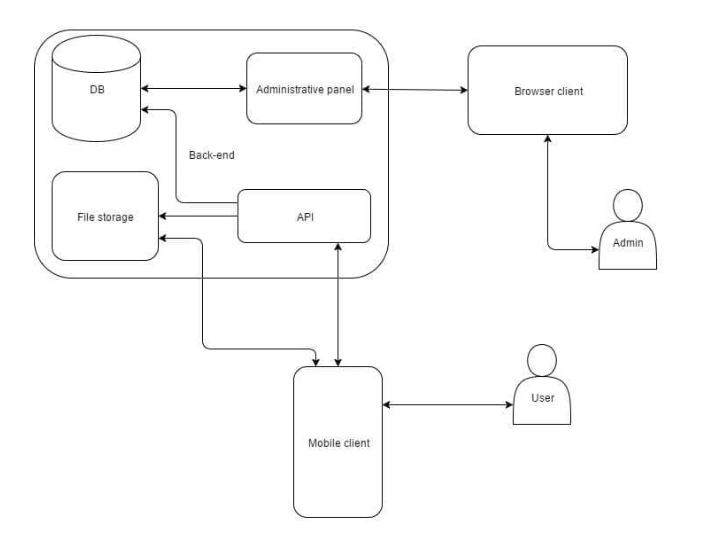
\includegraphics[width=1\textwidth]{img/architecture.png}
    \caption{Architecture}
    \label{fig:architecture}
\end{figure}

\newpage

As shown in Figure \ref{fig:FileStructure}, the file structure of the application consists of the following main folders: java, res and  assets. Inside the java directory are the main classes of the application (MainActivity, QRActivity, LibraryActivity). Inside the res directory are the resources of the application (icons, layouts, strings). Each layout represents a screen of the application (an Activity). Inside the assets directory are the \ac{3D} models their images and the tutorial for some of the models. The assets directory is read-only at runtime so in order to remove models from the application or to add new models, the application will copy the files from assets to the local smartphone storage.

As shown in Figure \ref{fig:Dependencies}, the build.gradle file contains the dependencies of the application. Also in the bottom of the figure is the method to generate a \textit{.sfb} file from a \textit{.obj} file. Sceneform supports 3D assets in the following formats:
\begin{enumerate}
    \item OBJ
    \item glTF (animations not supported)
    \item FBX, with or without animations.
\end{enumerate}
The models can be animated and also they can have textures and custom material\cite{Sceneform}.

\begin{figure}[ht]
    \begin{minipage}{0.5\textwidth}

        \begin{center}
            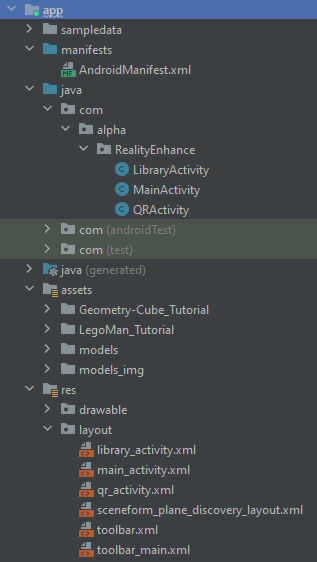
\includegraphics[width=0.65\textwidth]{img/File Structure.png}
            \caption{File Structure}
            \label{fig:FileStructure}
        \end{center}
    \end{minipage}
    \begin{minipage}{0.5\textwidth}
        \begin{center}
            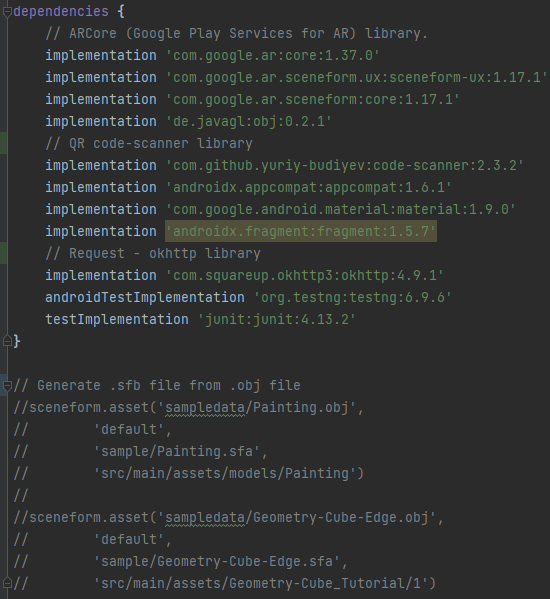
\includegraphics[width=1\textwidth]{img/Dependencies.png}
            \caption{build.gradle file}
            \label{fig:Dependencies}
        \end{center}
    \end{minipage}
\end{figure}




\clearpage

\section{Diagrams}
\subsection*{Class Diagram}
As shown in Figure \ref{fig:ClassDiagram}, the class diagram of the application consists of the following main classes: MainActivity, QRActivity and LibraryActivity.

The MainActivity class is the main class of the application. It is the first class called when the application is started, and it is responsible for the \ac{AR} mode. It contains methods dedicated to interacting with the \ac{3D} models (moving the model, rotating the model, scaling the model).

The QRActivity class is responsible for the \ac{QR} code reader. It has a method called when a \ac{QR} code is scanned and verifies if it is valid. It will check if the model is already imported. If the model is already imported, it will load it from the local storage; it will also request the Google Bucket Storage.

Lastly, the LibraryActivity class is responsible for the list of models and the loading of the models.
\begin{figure}[ht]
    \centering
    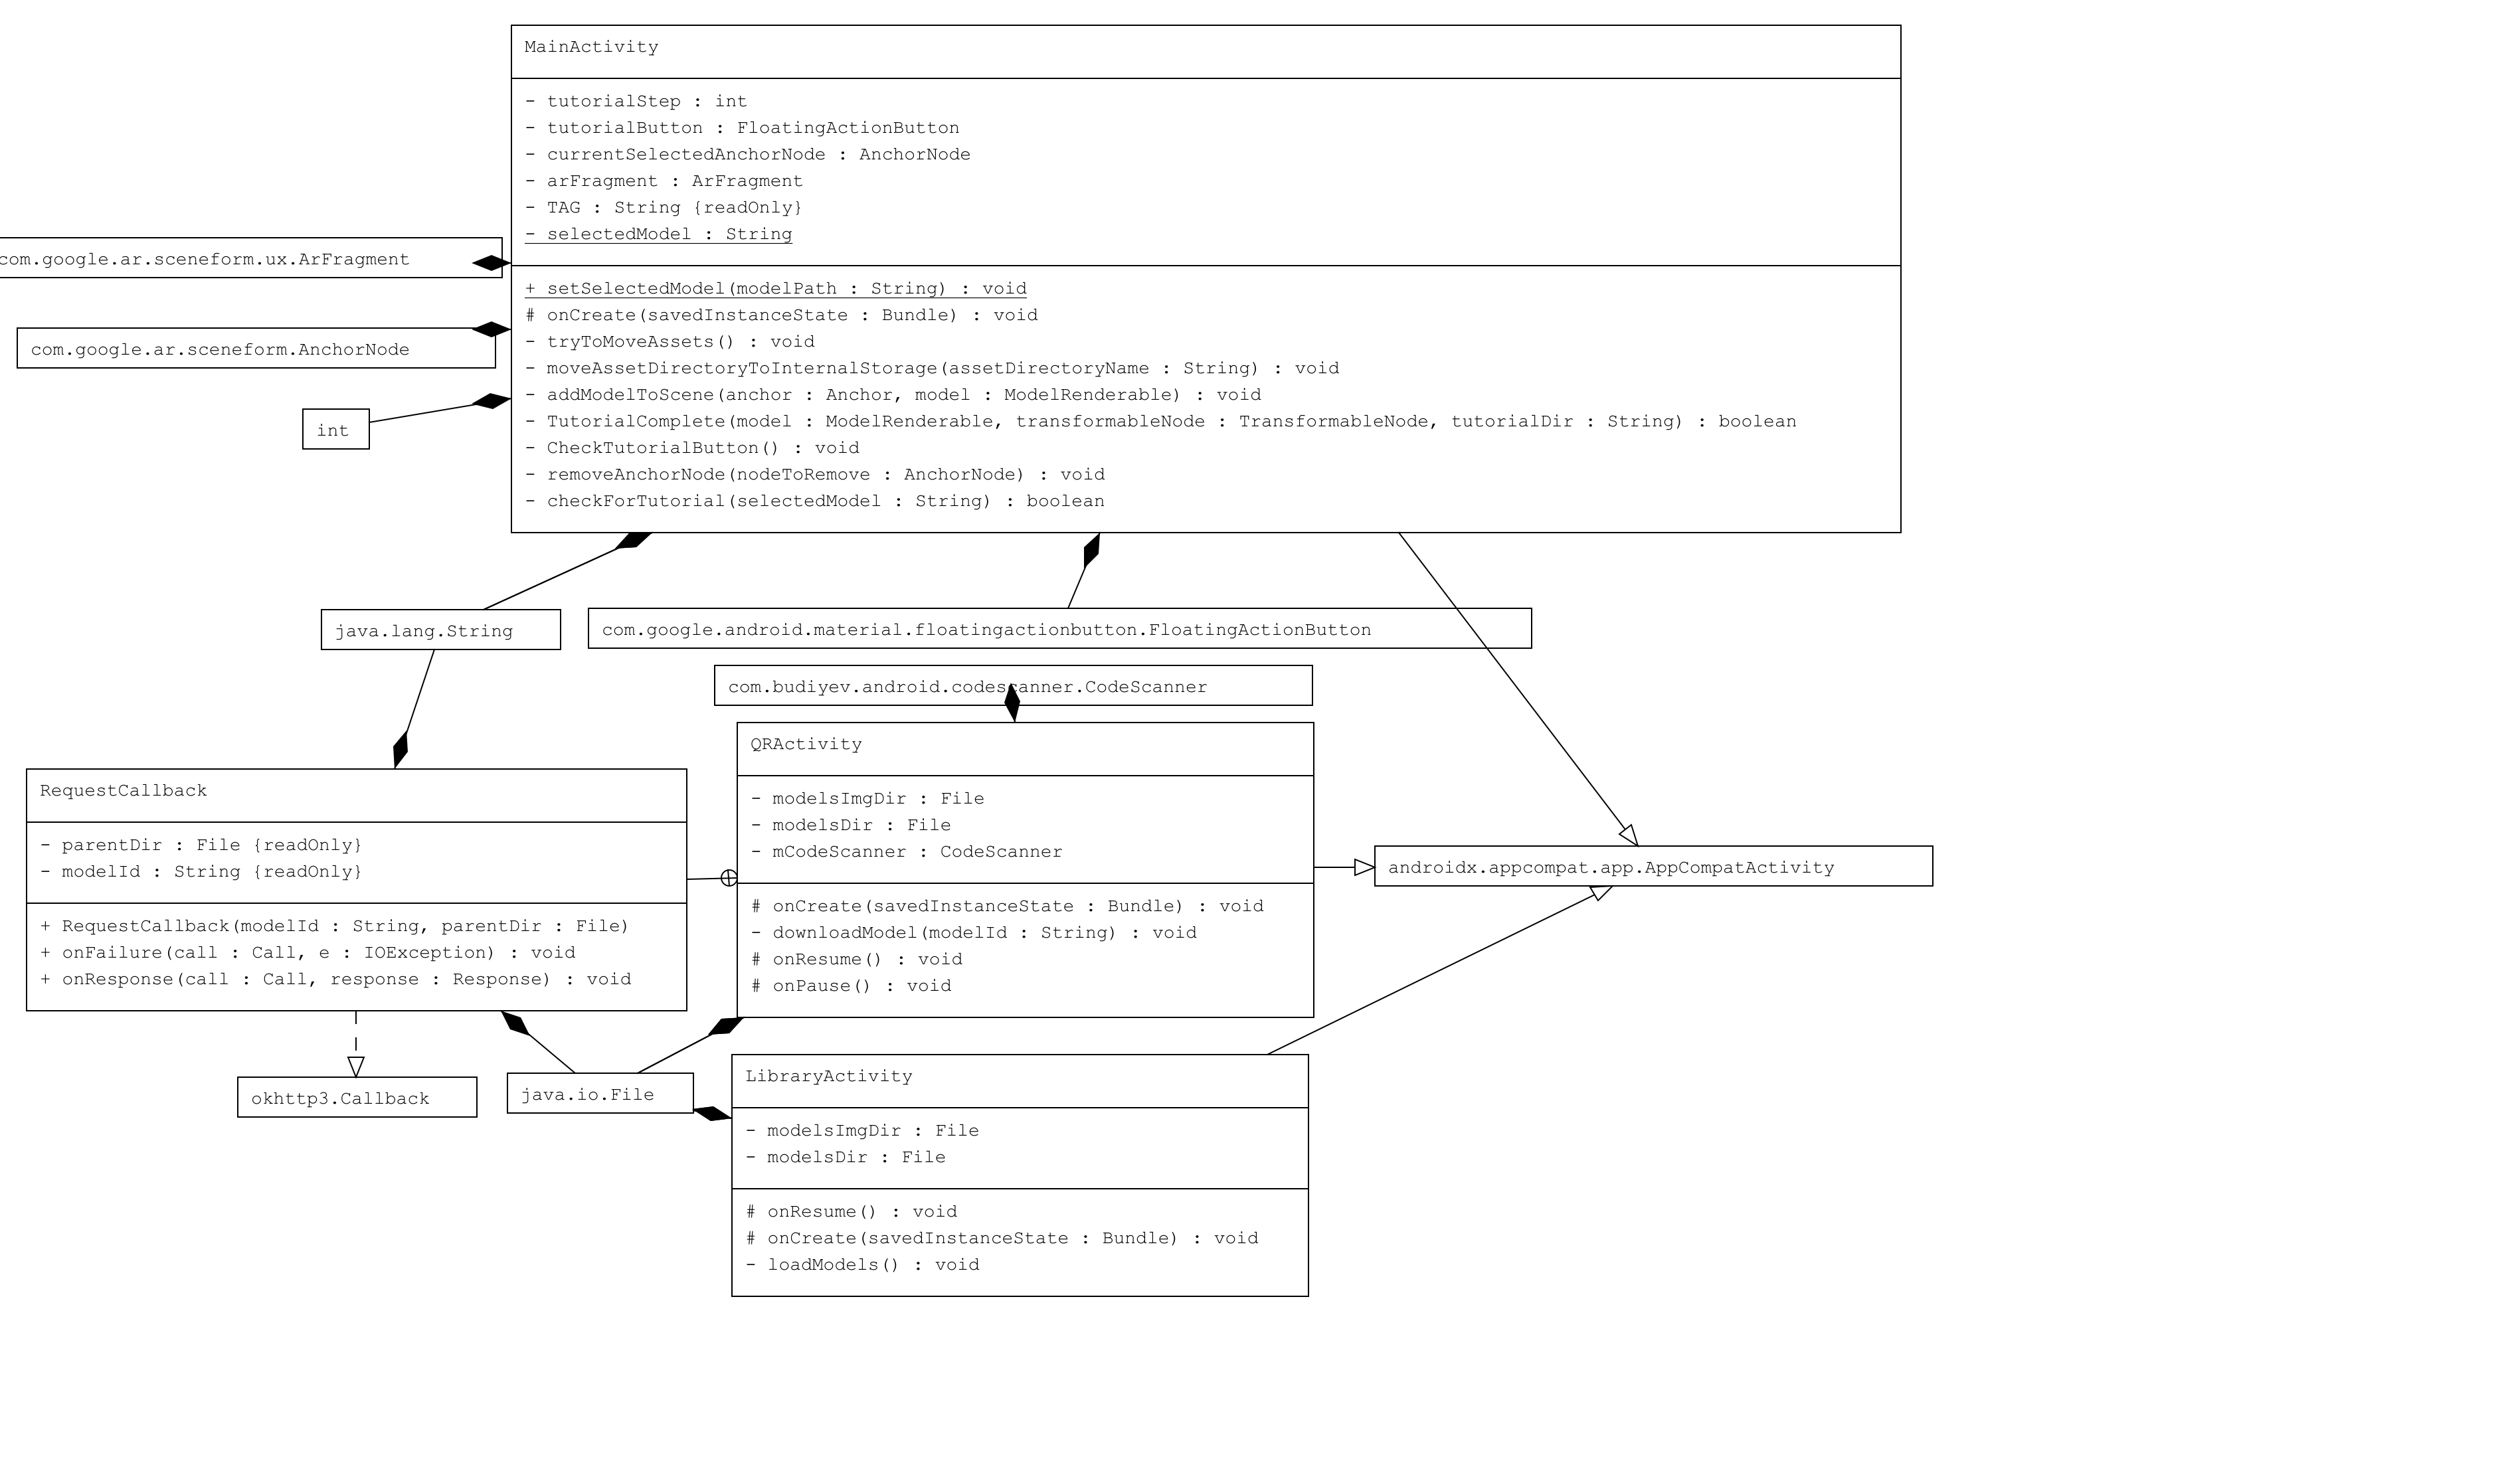
\includegraphics[height=0.9\textwidth]{img/ClassDiagram.png}
    \caption{Class Diagram}
    \label{fig:ClassDiagram}
\end{figure}


\subsection*{Use Case Diagram}
By looking at the Use Case Diagram in Figure \ref{fig:UseCaseDiagram}, we can see what the user is able to do inside the application. RealityEnhance allows the users to scan a \ac{QR} code load or to import a new model. It also gives users the power to interact with the \ac{3D} models in the \ac{AR} mode. The users can also browse a library of already imported models.

The ability to interact with the \ac{3D} models is a very important feature of the application. It allows the users to see the models from different angles and to change the size, orientation and position using familiar gestures. It also gives users the possibility to remove a selected model that is already placed in the \ac{AR} scene.
\begin{figure}[ht]
    \centering
    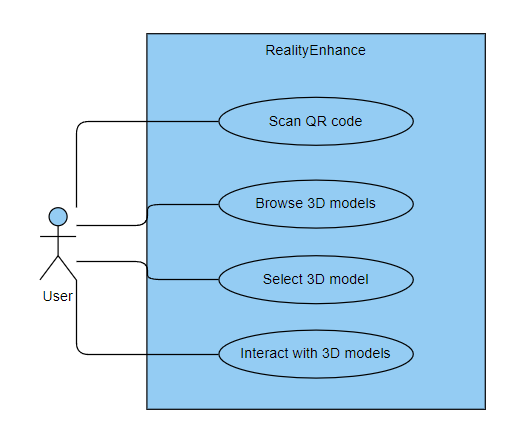
\includegraphics{img/UseCaseDiagram.png}
    \caption{Use Case Diagram}
    \label{fig:UseCaseDiagram}
\end{figure}

\clearpage

\subsection*{Sequence Diagram}
The Sequence Diagram in Figure \ref{fig:SequenceDiagram} shows the interaction between the user and the application. The user starts the application and is presented with a prompt that will request permission to use the camera. After that, the \ac{AR} module will begin to scan the user's surroundings in order to map the environment. For importing a new model, RealityEnhance uses a \ac{QR} code scanner that will check if the code is valid.
\begin{figure}[ht]
    \centering
    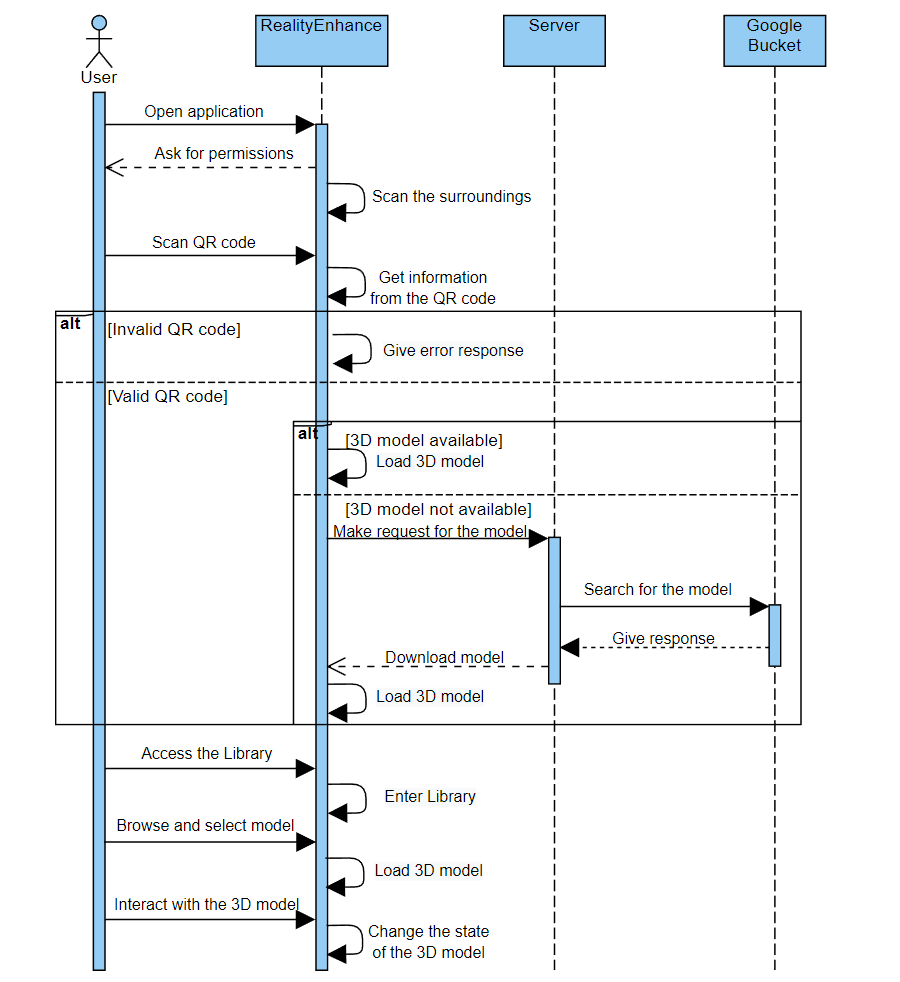
\includegraphics[width=1\textwidth]{img/SequenceDiagram.png}
    \caption{Sequence diagram}
    \label{fig:SequenceDiagram}
\end{figure}
\newpage

If the code fails the validation process, the user will be notified and will be prompted to scan another code. If the code is valid, the application will check if the model is already in the local storage, and it will load it. If the model is not in the local storage, the application will make a request to Google Bucket Storage to retrieve all the information about the model (model file, textures, model image, model guide/interactive guide). After the request is completed, a response will be sent back with all the information about the model. The model will then be saved in the local storage and loaded in the \ac{AR} scene.

The user can also browse the Library of already imported models. It also has access to the \ac{QR} scanner interface and can search for the desired model that is wanted to be loaded in the \ac{AR} scene.

The interaction between the user and the model bridges the virtual-physical gap and helps build a sense of immersion.

\newpage
\section{Publishing RealityEnhance}
\subsection*{Introduction to App Distribution Platforms}
App distribution platforms are used by developers to publish their applications, and the success of an application depends on the platform it is published on. The most popular platforms are Google Play Store and Apple App Store, and they play a crucial role in reaching a wide audience.

\subsection*{Google Play Store overview}
Google Play Store is the official app store for Android devices\cite{GooglePlay}, offering users a diverse range of applications across various categories. This distribution platform was selected for publishing RealityEnhance because the application was developed for Android devices.

Before publishing an application on Google Play Store, the developer must create a Google Play Console account. The Google Play Console is a platform that allows developers to publish and distribute their applications to Android users around the world. It also provides developers with tools to grow their user base and earn revenue. The Google Play Console is a web-based platform that can be accessed from any computer with a web browser. It is also available as an Android application.

The application needs to be prepared for release before it can be published on Google Play Store. The developer must have a specific file structure, shown in Figure \ref{fig:GooglePlayConsole}, and then create a signed bundle file. After the bundle file is created, the developer can upload it to the Google Play Console and publish the application.

\begin{figure}[ht]
    \centering
    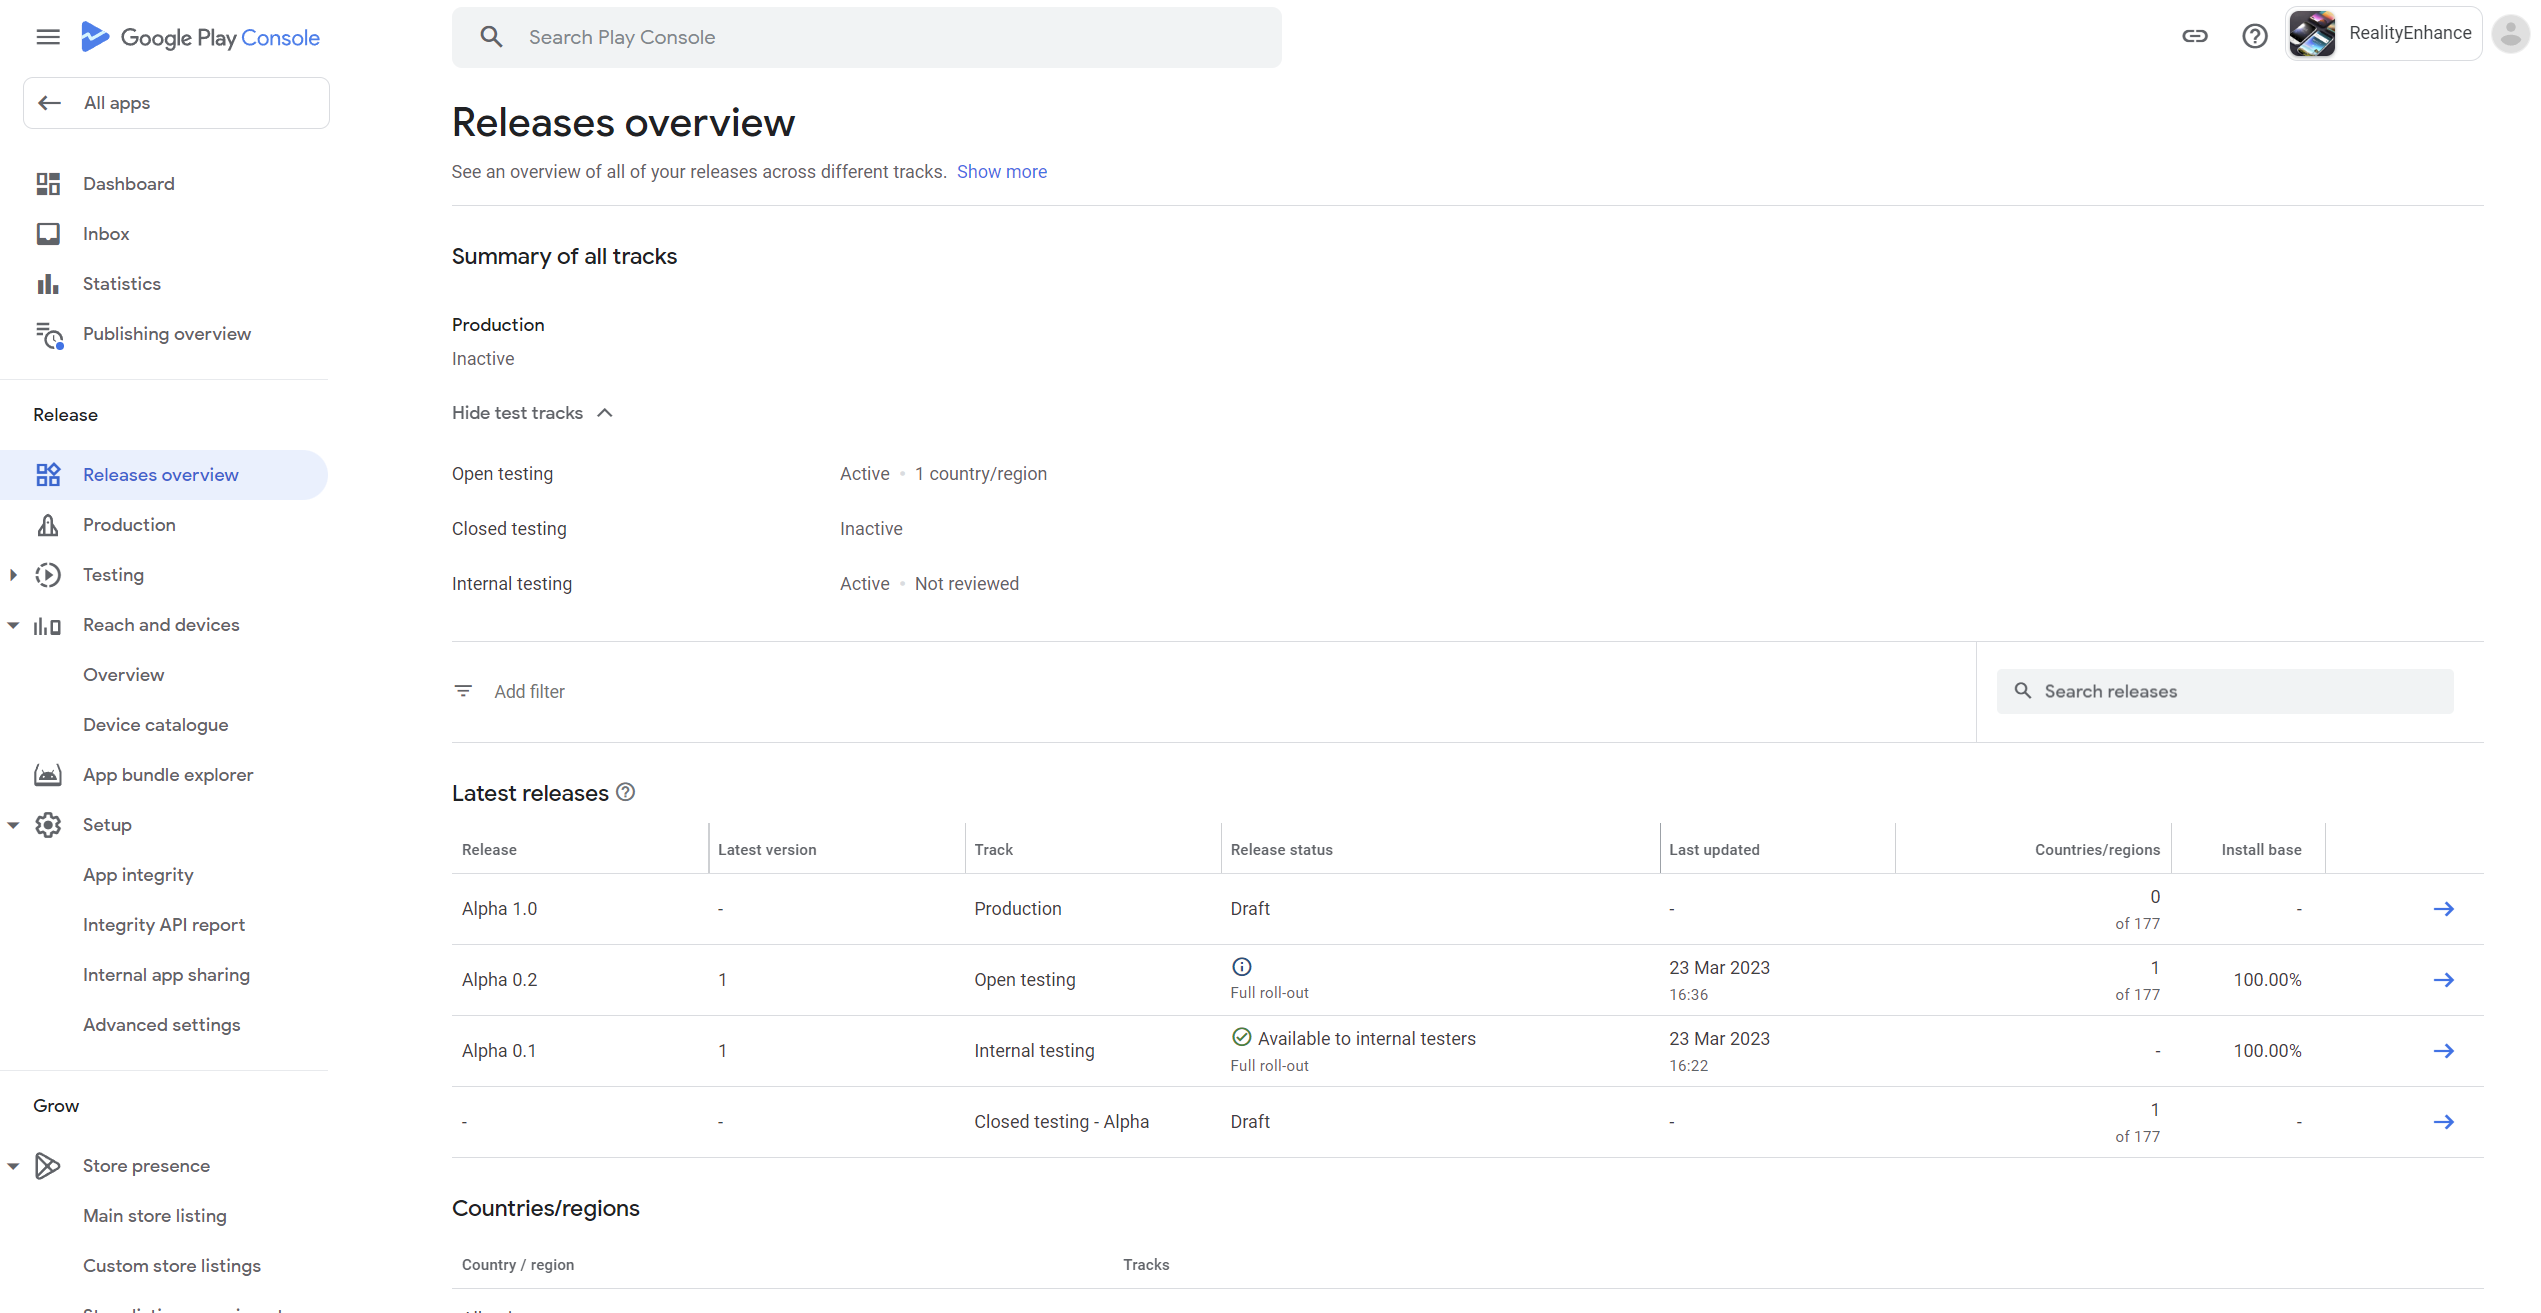
\includegraphics[width=1\textwidth]{img/GooglePlayConsole.png}
    \caption{Google Play Console}
    \label{fig:GooglePlayConsole}
\end{figure}